\chapter{Topic: Lindenmayer system}
{ }\hfill\textbf{Level:} Advanced\\ \\
\noindent
In this part, I take reference from:
\begin{itemize}
 \item  the english Wikipedia page about L-systems: \texttt{http://en.wikipedia.org/wiki/L-System}.
 \item the book ``The Algorithmic Beauty of Plants'' written by Przemyslaw Prusinkiewicz and Aristid Lindenmayer.
\end{itemize}
This section will deal with the Lindemayer systems or L-system introduced and developed in 1968 by the Hungarian theoretical biologist Lindenmayer. A L-System is a set of rules and symbols used to to model the growth processes of plant development, but also able to model the morphology of a variety of organisms. The main concept in L-Systems is ``rewriting rules''. This technic is used to replace some initial condition using some rules to do the replacement.
\section{Formal definition}
\noindent
A L-System is a formal grammar with :
\begin{enumerate}
 \item An alphabet $V$ : The set of the variables of the L-System. $V *$ stands for the set of the ``words'' we could generate with any symbols taken from alphabet $V$, and $V +$ the set of ``words'' with at least one symbol.
 \item A set of constant values $S$. Some of this symbol are common to all L-System. (in particular with the turtle!).
  \item A start awiom $\omega$ taken from  $V +$ , it is the initial state.
 \item A set of prodution rules $P$ of the $V$ symbols.
\end{enumerate}
Such a L-System is defined as a tuple $\{V,S,\omega,P\}$.\\ \\
Let's consider the following L-system:
\begin{itemize}
 \item Alphabet : $V = \{A, B\}$
 \item Constants : $S = \{\emptyset\}$
 \item Start Axiom: $\omega = A$
 \item Rules : $\begin{array}{|l|}
\hline
A \rightarrow AB \\
B \rightarrow A \\ 
\hline
\end{array}
$
\end{itemize}
The two production rules are rewriting rules. On each step, the symbol $A$ is replaced by the séequence $AB$, and the symbol $B$ is replaced by $A$. Here are the first iterations of this Lindemayer system:
\begin{center}
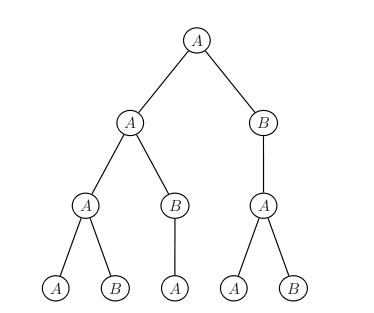
\includegraphics[width=8cm]{pics/linden-arbre.png}
\end{center}
\begin{itemize}
\item Itération 1: $A$
\item Itération 2: $AB$
\item Itération 3: $ABA$
\item Itération 4: $ABAAB$
\end{itemize}
\vspace*{0.2cm}
Ok, ok but concretely? Let's read next section!
\section{Turtle interpretation}
\noindent This first example helps to understand what is a Lindenmayer system but we can't see for now the rapport with our turtle and \logo..\\ \\
Here it comes interesting: every word we built before has no meaning. We're going to define for each letter of the sequence an action to execute with the turtle, and draw with this method 2D or 3D drawing.
\subsection{Usual Symbols}
\begin{itemize}
 \item $F$ : Forward one unit step ($\in V$)
 \item $+$ : Turns left angle $\alpha$ $(\in S)$.
 \item $-$ : Turns right angle $\alpha$ $(\in S)$.
 \item $\&$ : Go down angle $\alpha$ $(\in S)$.
 \item \textasciicircum : Go up angle $\alpha$ $(\in S)$.
 \item \textbackslash: Roll left angle $\alpha$ $(\in S)$.
 \item $/$: Roll right angle $\alpha$ $(\in S)$.
 \item $|$: Half-tour. In \xlogo: \texttt{rt 180}
\end{itemize}
\vspace*{0.2cm}
For example, if $\alpha=90$ with a unit step of 10 turtle steps, we have:
\begin{center}
 \begin{tabular}{|c|c|c|c|c|c|c|c|c|}
 \hline
Symbol & $F$ & $+$ & $-$ & $\&$ & \textasciicircum & \textbackslash& $/$ & $|$ \\
 \hline
\xlogo\ Command & \texttt{fd 10}&\texttt{lt 90}&\texttt{rt 90}&\texttt{down 90}&\texttt{up 90}&\texttt{lr 90}&\texttt{rr 90}&\texttt{rt 180}\\
 \hline
\end{tabular}
\end{center}
\subsection{Van Snowflake}
Let's consider the L-system:
\begin{itemize}
 \item [\textbullet] Initial state: $F--F--F--$
 \item [\textbullet] Production rules: $F \rightarrow F+F--F+F$
 \item [\textbullet] Angle $\alpha=60$\degre, Unit step is divided by 3 between each iteration.
\end{itemize}
First iterations:
\begin{center}
\begin{minipage}{7.5cm}
 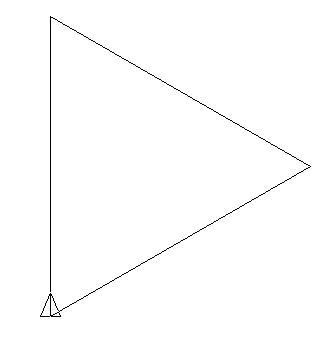
\includegraphics[width=7.5cm]{pics/linden-flocon1.png}
\end{minipage}
\begin{minipage}{7.5cm}
 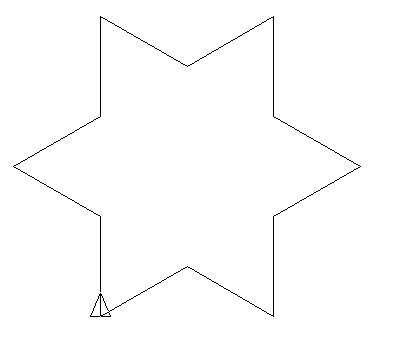
\includegraphics[width=7.5cm]{pics/linden-flocon2.png}
\end{minipage}\\
\begin{minipage}{7.5cm}
 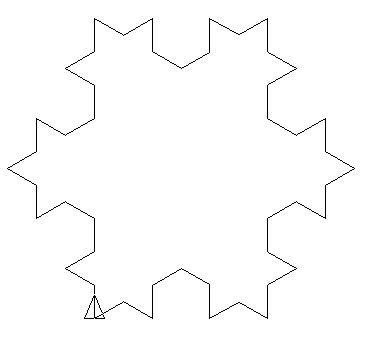
\includegraphics[width=7.5cm]{pics/linden-flocon3.png}
\end{minipage}
\begin{minipage}{7.5cm}
 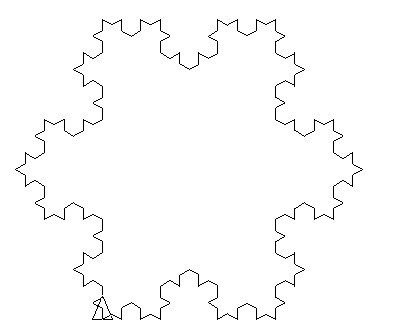
\includegraphics[width=7.5cm]{pics/linden-flocon4.png}
\end{minipage}
\end{center}
\noindent \xlogo Program:
\begin{verbatim}
 
to snowflake :p
globalmake "unit 300/power 3 :p-1
repeat 3 [f :p-1 right 120]  
end

to f :p
if :p=0 [forward :unit stop]
f :p-1 left 60 f :p-1 right 120 f :p-1 left 60
f :p-1 
end

\end{verbatim}
\subsection{Quadratic Van Koch curve}
\noindent Given this new L-system:
\begin{itemize}
 \item[\textbullet] Initial state: $F-F-F-F$
 \item[\textbullet] Production rules: $F\rightarrow F-F+F+FF-F-F+F$
\end{itemize}
Here are the first representations using $\alpha=90$, we adjust the unit step for the figure has a constant size.
\begin{center}
\begin{minipage}{7.5cm}
 
\includegraphics[width=7.5cm]{pics/linden-koch1.png}
\end{minipage}
\begin{minipage}{7.5cm}
 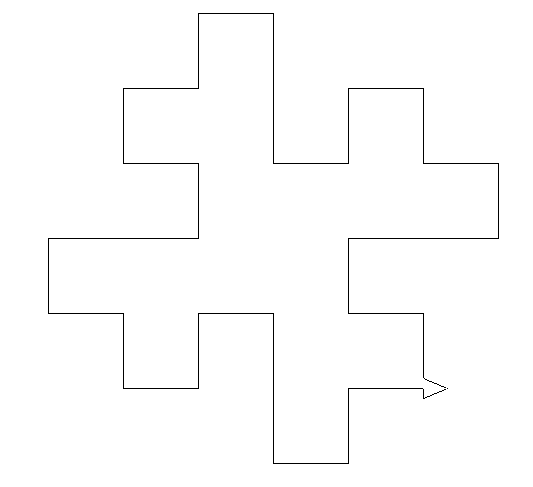
\includegraphics[width=7.5cm]{pics/linden-koch2.png}
\end{minipage}\\
\begin{minipage}{7.5cm}
 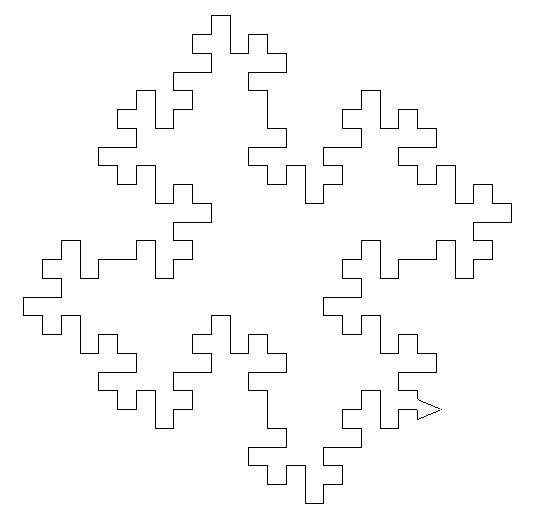
\includegraphics[width=7.5cm]{pics/linden-koch3.png}
\end{minipage}
\begin{minipage}{7.5cm}
 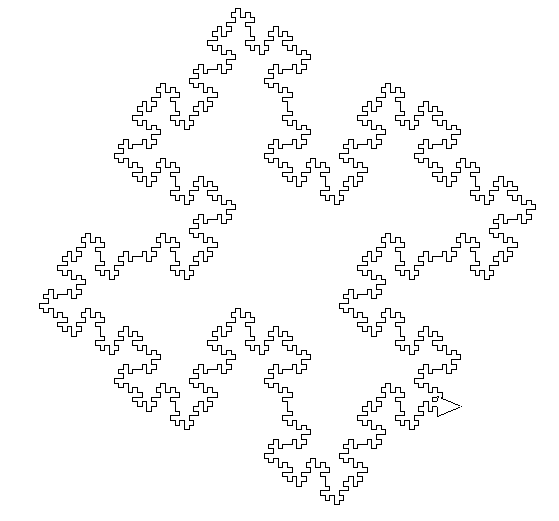
\includegraphics[width=7.5cm]{pics/linden-koch4.png}
\end{minipage}
\end{center}
Then it is very easy to create a Logo program to generate these drawings:
\begin{verbatim}
# p represent the order
to koch :p
# Between two iteration, the unit step is divided by  4
# The final figure will have a maximal size of 600x600 
globalmake "unit 300/power 4 :p-1

repeat 3 [f :p-1 left 90] f :p-1 
end

# Rewriting rules
to f :p
if :p=0 [forward :unit stop]
f :p-1 left 90 f :p-1 right 90 f :p-1 right 90
f :p-1 f :p-1 left 90 f :p-1 left 90 f :p-1 right 90 f :p-1
end
\end{verbatim}
\subsection{Dragon curve}
\begin{itemize}
 \item[\textbullet] Initial state: $F$\\
 \item[\textbullet] Production rules: $\begin{array}{|l|}
\hline
A\rightarrow A+B+ \\
B\rightarrow -A-B \\
\hline
\end{array}$ 
\end{itemize}
\begin{verbatim}
to a :p
if :p=0 [forward :unit stop]
a :p-1 left 90 b :p-1 left 90
end

to b :p
if :p=0 [forward :unit stop]
right 90 a :p-1 right 90 b :p-1

end

to dragon :p
globalmake "unit 300/8/ :p  
a :p
end
\end{verbatim}
\begin{center}
 \begin{minipage}{7cm}
 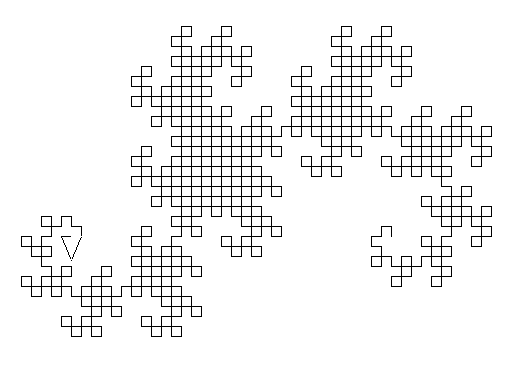
\includegraphics[width=7cm]{pics/linden-dragon10.png}
 \begin{center}
  \texttt{dragon 10}
 \end{center}
\end{minipage}
 \begin{minipage}{7cm}
 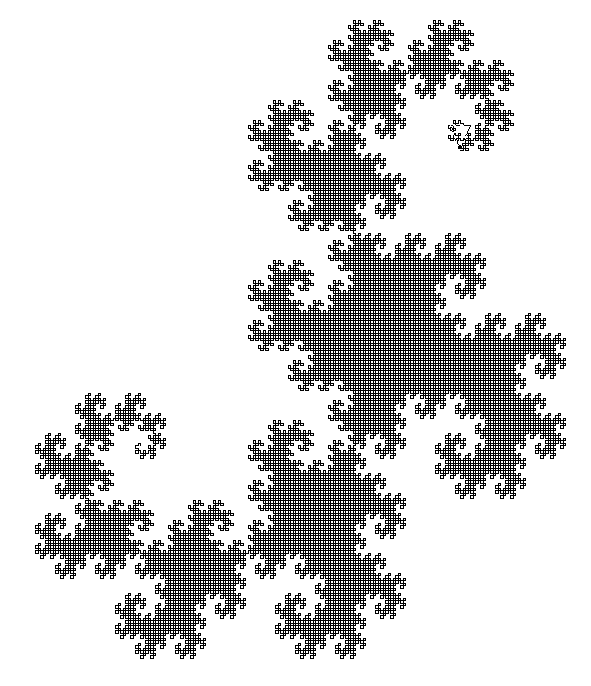
\includegraphics[width=7cm]{pics/linden-dragon15.png}
 \begin{center}
  \texttt{dragon 15}
 \end{center}
\end{minipage}
\end{center}

\subsection{Hilbert 3D curve}
\noindent The following example will generate a 3D Hilbert curve. This curve is singular because it fills perfectlty a cube when we increase iterations.\\ \\
Here is the L-system to consider:
\begin{itemize}
 \item Initial state: $A$
 \item Angle $\alpha=90$\degre, Unit step is divided by 2 between two iterations.\\
 \item Production rule: $\begin{array}{|l|}
\hline
A\rightarrow B-F+CFC+F-D\&F \textrm{\textrm{\textasciicircum}} D-F+\&\&CFC+F+B// \\
B\rightarrow A\&F\textrm{\textrm{\textasciicircum}} CFB\textrm{\textasciicircum} F \textrm{\textasciicircum} D\textrm{\textasciicircum} \textrm{\textasciicircum}-F-D\textrm{\textasciicircum}|F\textrm{\textasciicircum} B|FC\textrm{\textasciicircum} F\textrm{\textasciicircum} A// \\
C\rightarrow|D\textrm{\textasciicircum}|F\textrm{\textasciicircum} B-F+C\textrm{\textasciicircum} F\textrm{\textasciicircum} A\&\&FA\&F\textrm{\textasciicircum} C+F+B\textrm{\textasciicircum} F\textrm{\textasciicircum} D// \\
D\rightarrow|CFB-F+B|FA\&F\textrm{\textasciicircum} A\&\&FB-F+B|FC// \\
\hline
\end{array}$
\end{itemize}
\begin{verbatim}
to hilbert :p
clearscreen 3d
globalmake "unit 400/power 2 :p
linestart setpenwidth :unit/2
a :p
lineend
view3d
end

to a :p
if :p=0 [stop]
b :p-1 right 90 forward :unit left 90  c :p-1 forward :unit c :p-1
left 90 forward :unit right 90 d :p-1 downpitch 90 forward :unit uppitch 90 d :p-1
right 90 forward :unit left 90 downpitch 180 c :p-1 forward :unit c :p-1
left 90 forward :unit left 90 b :p-1 rightroll 180
end

to b :p
if :p=0 [stop]
a :p-1 downpitch 90 forward :unit uppitch 90 c :p-1 forward :unit b :p-1 uppitch 90 
forward :unit uppitch 90 d :p-1 uppitch 180 right 90 forward :unit right 90 d :p-1 
uppitch 90 right 180 forward :unit uppitch 90 b :p-1 right 180 forward :unit c :p-1 
uppitch 90 forward :unit uppitch 90 a :p-1 rightroll 180 
end

to c :p
if :p=0 [stop]
right 180 d :p-1 uppitch 90 right 180 forward :unit uppitch 90 b :p-1 right 90
forward :unit left 90 c :p-1 uppitch 90 forward :unit uppitch 90 a :p-1 downpitch 180
 forward :unit a :p-1 downpitch 90 forward :unit uppitch 90 c :p-1 left 90 forward :unit 
left 90 b :p-1 uppitch 90 forward :unit uppitch 90 d :p-1 rightroll 180 
end

to d :p
if :p=0 [stop]
right 180 c :p-1 forward :unit b :p-1 right 90 forward :unit left 90 b :p-1 right 180
forward :unit a :p-1 downpitch 90 forward :unit uppitch 90 a :p-1 downpitch 180 forward :unit
b :p-1 right 90 forward :unit left 90 b :p-1 right 180 forward :unit c :p-1 rightroll 180
end
\end{verbatim}
And the first iterations:
\begin{center}
\begin{minipage}{7cm}
 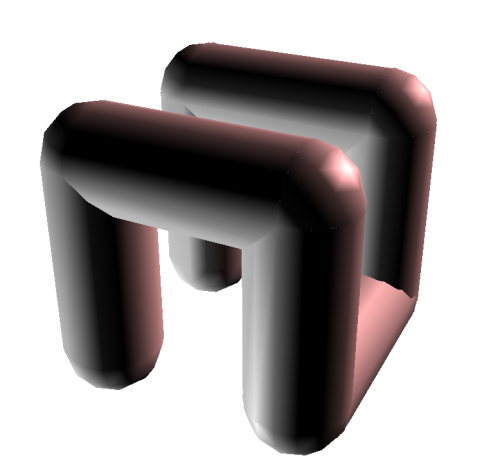
\includegraphics[width=7cm]{pics/linden-hilbert1.png}
\end{minipage}
\begin{minipage}{7cm}
 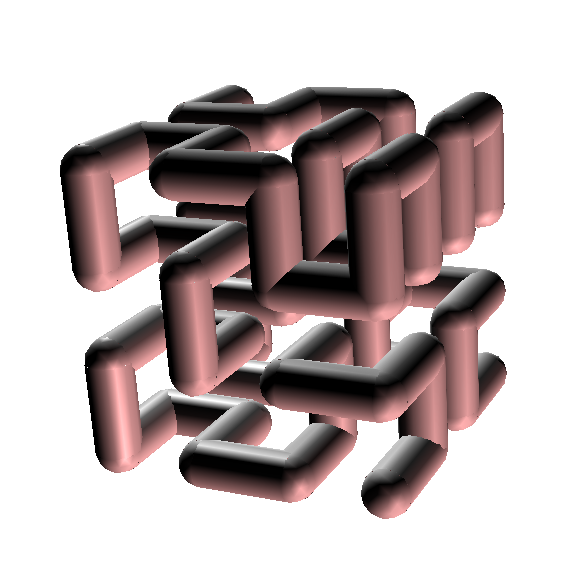
\includegraphics[width=7.5cm]{pics/linden-hilbert2.png}
\end{minipage}\\
\begin{minipage}{7cm}
 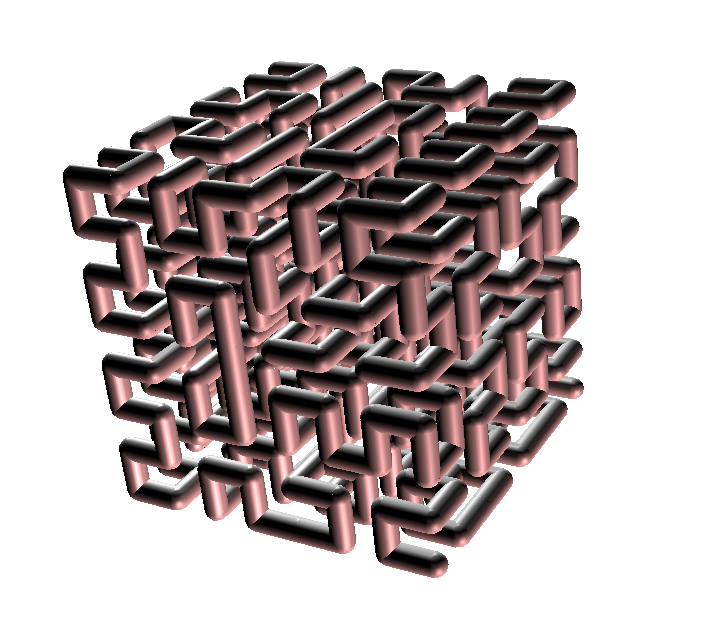
\includegraphics[width=7cm]{pics/linden-hilbert3.png}
\end{minipage}
\begin{minipage}{7cm}
 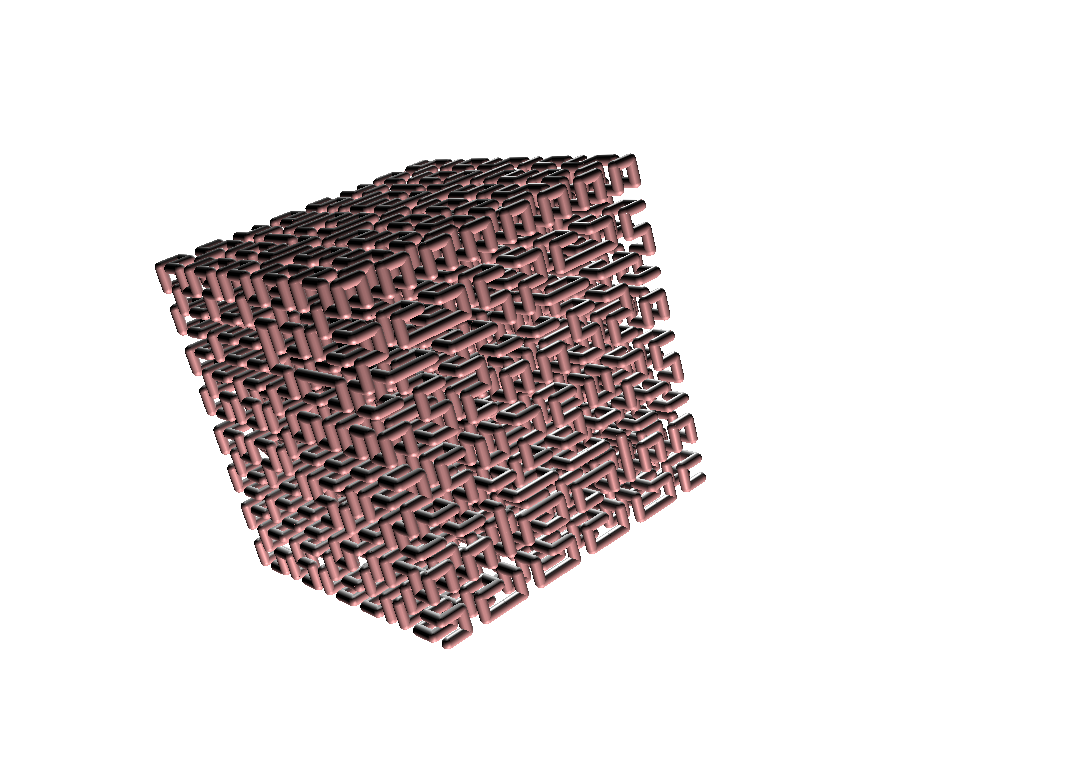
\includegraphics[width=9cm]{pics/linden-hilbert4.png}
\end{minipage}
\end{center}
Nice, isn't it?